% !TEX root = ../thesis.tex
%
\chapter{Design and Implementation}
\label{ch:implementation}

This chapter describes details about the design, implementation, and configuration of \acf{IFAS}.
Appendix \cref{ch:appendix:source} contains the source code of the services and applications as they are mentioned over the course of this chapter.
The full source code is available via GitHub\footnote{\url{https://github.com/janis-kra/master-impl}}\todo{link to "final" tag when done}.
%At the time of beginning the implementation, the current Elasticsearch and Kibana versions were 6.1.1, the current Event Store version was 4.1.

%After consideration of the goals for the \acf{IFAS} and the results from the classifications made earlier (cf. \cref{ch:classifications}), the system was designed.
%This activity includes specific decisions such as which data to collect and especially how to implement the Event Store-Elasticsearch bridge service, as well as working out the overall architecture of the whole system.

\section{Client Application}
\label{sec:implementation:client}

The Mattermost web application was extended with custom code in order to send user feedback.
This section first discusses the problems with implementing sending of implicit user feedback in web applications and then briefly explains how the actual implementation was done.

\subsection{Challenges with reliable feedback sending}
\label{subsec:implementation:client:problems}

When tracking user interactions in a web application, the technical idiosyncrasies of reliably sending data via \ac{XHR} requests using JavaScript can become problematic.
This is explained in this section via the concrete example of click tracking.
For various reasons, which are discussed below, there are no valid alternatives to doing asynchronous \ac{XHR} requests for click tracking for this use case though.

The gist of the problem is that when a user clicks a link in a web application, this normally introduces a redirect to a new page, therefore potentially aborting the asynchronous \ac{XHR} request~\cite{Kohavi2010}.
This problem could be solved by doing a synchronous request instead of an asynchronous one, but this is not a desirable solution because the whole web application would block for the duration of the request.
If the user's internet connection is slow -- e.g .when accessing the application on a mobile phone -- or the logging server is experiencing heavy load, this can introduce a noticeable and annoying delay.
These delays can be a reason to make the user abandon the application altogether~\cite{Kohavi2010,Dmitriev2017}.

In order to mitigate these problems, the Navigator \ac{API} of modern browsers was extended with the \texttt{sendBeacon}\footnote{\url{https://developer.mozilla.org/en-US/docs/Web/API/Navigator/sendBeacon}} method, but this cannot be used for this use case for two reasons.
The concept of the \texttt{sendBeacon} method is that it can be used to asynchronously send a small amount of data to a server prior to the user leaving the page, in a reliable way.
However, this is not implemented yet in all modern browsers\footnote{\url{https://caniuse.com/\#feat=beacon}}, especially Internet Explorer and the desktop and mobile Safari browsers.
Also, when posting data to Event Store using its \ac{HTTP} \ac{API}, the \texttt{ES-EventId} header has to be attached to the request with a unique id -- attaching custom headers via the \texttt{sendBeacon} method is not supported though.

Another possibility for delivering implicit user feedback is the web beacon technique, which work by sending a request for a special 1x1 pixel image on a server.
While this was a very popular method a few years ago, improvements in web browser and the JavaScript language make web beacons rather outdated.
\citet{Kohavi2012} report additional problems with browsers aborting requests made via the web beacon technique.
Thus, web beacons are not a suitable alternative for sending the feedback to the server.

For the reasons discussed above, a standard asynchronous \ac{XHR} is the best alternative.
This would introduce click data being lost when the request is dropped, but as the Mattermost chat application used as the client here is a \ac{SPA}, this is not a problem.

Technically, there exist three different click event types: \texttt{mousedown}, \texttt{mouseup} and \texttt{click}.
Capturing the event on \texttt{mousedown} would cause the event to fire earlier than the two other event types, but this is not necessary as problems with lost click events are not expected because Mattermost is a \ac{SPA}.

\subsection{Feedback Sending Module}

A small JavaScript module was implemented, which exports a function for sending the feedback data.
The source code is listed in the appendix under \cref{appendix:code:implementation:mattermost:feedbackjs}.

The feedback module exports one function, \texttt{initFeedback}, which takes a URL and a stream name as arguments.
This function's return value is another function, called \texttt{feedback}, that sends the actual user feedback for a given event type.
The \texttt{feedback} function sets the appropriate \ac{HTTP} headers and creates a unique id for the event, then sends the \ac{XHR} request to the Event Store at the URL previously set via \texttt{initFeedback}.
This generic approach makes the module universally applicable for any client application that is written in JavaScript.

The feedback module is used in various places throughout the Mattermost web application in order to send the user feedback as specified in \cref{sec:design:event-structure}.
For most types of user feedback, additional data from the application's internal state was required.
This was obtained via various \ac{API} functions provided by Mattermost.

\section{User Feedback Events}
\label{sec:design:event-structure}

User feedback is sent to \ac{IFAS} in the form of events, as the data is internally first saved in \ac{IFAS}' Event Store.
All events are saved to a single Event Store stream; this helps to isolate the user feedback data separated from other data that may be posted to Event Store in a production environment.

In order to supply the data that is necessary for the metrics defined earlier, five different event types were created.
These event types are listed below, together with a description of the data that they provide and in which cases they are sent to \ac{IFAS}:

\begin{description}
\item[ChannelSwitched]
Whenever a user switches the messaging channel, this event is sent.
It contains data about the channel that is switched to, as well as the method of channel switching: Via the left-side menu bar, or via the \emph{channel switcher} feature.
\item[TutorialExperimentParticipated]
This event contains information about the decision a newly registered user makes regarding the Mattermost tutorial:
Either the user participates in the tutorial, or they skip it.
As this event is used as the data source for an A/B test, it also contains information about the group that the user was assigned to, which is either control or treatment.
\item[PostCreated]
Every time a message is sent in Mattermost, a new \texttt{PostCreated} event is fired.
This event contains extensive data about the message itself, such as its contents and the sender's id, as well as a lot of metadata such as the channel the message was posted to and the time it was created.
The resulting data is used to compute the metric regarding active channel usage.
\item[UserClicked]
These events are used to capture all clicks that a user performs in the application.
The intention is that for any application, these events give an analyst enough information to identify what the user was doing at any given point.
The \texttt{UserClicked} event contains information about the clicked element such as the HTML attributes \texttt{class} and \texttt{id} as well as its inner text.
There may still be cases where this is not enough to identify the action that the user performed, which is why the event is amended with the click's position within the application, the window's height and width, and the current URL.
Using this information, the analyst can exactly identify the position where the user clicked at the given point in time.
\item[WindowScrolled]
Whenever a user scrolls up or down in the chat window, a \texttt{WindowScrolled} event is sent to \ac{IFAS}.
This event encaspulates information about the URL at which the scrolling occured, as well as the duration and amount of the scrolling.
Using this event's data, the scrolling amount metric can be computed.
\end{description}

Parts of the data contained in these events may be redundant or unspecific in some cases, but helps to recreate the user's steps if this is needed.
The additional data could also be used to later measure additional metrics.
%If this is undesirable because the additional data takes up too much disk space, or because of moral concerns regarding the hoarding 
In a production environment, the specificity of these events could be improved by assigning unique ids to every element in the web application, or at least to the ones which are of special interest.
Especially the \texttt{UserClicked} events would benefit from this.

\section{Event Store Configuration}
\label{sec:implementation:storage}

The storage layer of \ac{IFAS} is realized by Event Store.
An officially maintained Docker image\footnote{\url{https://hub.docker.com/r/eventstore/eventstore/}} is used as the starting point and requires little additional configuration.
At the time of implementation, the current Event Store version was 4.1.0.

The Event Store service definition is contained in the Compose file printed in the appendix under \cref{appendix:code:docker:docker-compose}.
This configuration starts up an Event Store container with mostly default settings, which exposes port 2113 in order to allow the client application to send events over the \ac{HTTP} interface.
In order to not lose critical data when a container is removed, two volumes \texttt{eventstoredata} and \texttt{eventstoreconfig} are created and mounted to the respective folders within the container's file system.
This stores the data and configuration in separate Docker volumes, which are preserved when the container is removed, which would be the case for example if a new version of the Event Store image is used.

This service definition also makes the Event Store's \ac{TCP} and \ac{HTTP} interfaces available via ports 1113 and 2113 for all services in the \texttt{IFAS-net} network.
The container can be accessed by other containers via its name, \texttt{eventstore}.
Thus, the bridge to the aggregation service (cf. \cref{sec:implementation:bridge}) listens to new events via the \ac{TCP} address \url{tcp://eventstore:1113}.
The client application however has to post events to the publicly available URL because it is not part of the \texttt{IFAS-net} network; in the case where both \ac{IFAS} and the client are run on the same machine the URL is \url{http://127.0.0.1:2113}.

\section{Event Store-Elasticsearch Bridge}
\label{sec:design:bridge}
\label{sec:implementation:bridge}

In order to move the event data to Elasticsearch and afterwards into Kibana, a service is needed which bypasses the lack of a direct integration of Event Store and Elasticsearch.
This service is the Event Store-Elasticsearch bridge (short just ``bridge'' in this context).

\subsection{The Need for a Bridge Service}

Intuitively, it seems problematic that Event Store and Elasticsearch have different concepts of storing their data.
On the one hand, Event Store data is stored as events in streams; each event always has an event type and a unique id within that stream.
On the other hand, in Elasticsearch, data is managed in indices which contain documents; each Elasticsearch document is assigned a document type.

The bridge spans the gap between the two concepts by subscribing to all events that are posted to the user feedback stream and posting them to Elasticsearch.
As Elasticsearch does not allow multiple document types in the same index since the release of the most recent major version\footnote{\url{https://www.elastic.co/guide/en/elasticsearch/reference/current/removal-of-types.html}}, each event type has to have its own Elasticsearch index.
Thus, \ac{IFAS} in its current state has five Elasticsearch indices, one for each event type.
The index names always have the Event Store stream's name as the prefix and the event type as the suffix, divided by an underscore.
In conclusion, each stream maps to the prefix of an index, each event type maps to the suffix of an index, and each event maps to a document (cf. \cref{table:design:bridge}).
The event type is automatically also the document type.

%This is also benefical for later analysis in Kibana, as indices with multiple document types would clutter the \ac{UI}

\begin{table}[ht]
\centering
\caption{Mapping of Event Store to Elasticsearch data types.}
\label{table:design:bridge}
\begin{tabular}{l|l}
\textbf{Event Store} & \textbf{Elasticsearch} \\ \cline{1-2}
Stream & Index prefix \\
Event type & Index suffix \& document type \\
Event & Document
\end{tabular}
\end{table}

One possible and seemingly convenient solution would be using Logstash\footnote{\url{https://www.elastic.co/products/logstash}} as the bridge, which is not applicable in this exact scenario though.
Logstash is another application from the Elastic stack; it serves the exact purpose to integrate data from various sources into Elasticsearch.
It is possible to consume Atom feeds via Logstash's \ac{RSS} plugin, which Event Store offers an interface for.
This is not feasible in this scenario as Logstash's \ac{RSS} plugin is not able to handle feeds which require authentication, which Event Store does.
Also, Event Store's persistent subscriptions are not compatible with Atom feeds, which is another reason to abandon Logstash as a possible solution.

Instead of using an existing service that listens to Atom feeds such as Logstash, a custom implementation is the better approach here.
This is the case because the official .NET Core Event Store client \ac{API}\footnote{\url{https://github.com/EventStore/ClientAPI.NetCore}} can be used, which allows amongst others for usage of persistent subscriptions and more efficient communication over a dedicated protocol built on top of \ac{TCP}.
The \ac{TCP} protocol variant is faster than the alternative via Atom feeds, which is built on top of \ac{HTTP}~\cite{WEB:EvtSt-Which-Api}.
It should be noted that, although using \ac{TCP} instead of \ac{HTTP} contradicts the requirement for an \ac{HTTP} interface as stated in \cref{sec:design:goals}, this is not a problem at all due to the heterogenous technology that a microservice architecture allows~\cite[Key Benefits,pp.~4f]{newman2015building}.

Assuming the Event Store stream already exists, setting up the bridge to transfer new events to an Elasticsearch index would then be a two-step process.
First, a persistent subscription has to be created within the Event Store administration overlay.
Then, an instance of the bridge service has to be started, configured to listen to the newly created subscription.
This would cause the bridge to transfer all existing events which were not read previously to the respective Elasticsearch indices, and then also posting all subsequently received events to this index.

It would also be possible to implement the bridge in a way that allows the service to listen to multiple subscriptions simultaneously.
This would require a more complex service which introduces two problems.
First, it introduces an unnecessary implementation overhead, and second, its additional complexity could lead to scaling problems.
Writing complex, large serices is in general discouraged to do in a microservice architecture~\cite[Key Benefits,pp.~5f]{newman2015building}.
Instead, multiple instances of the same service should be executed alongside each other, with their respective configuration for listening to a specific stream.

Thanks to persistent subscriptions, it is possible to temporarily take the bridge instance offline -- as the subscription state is persisted on the server side, the bridge can transfer all events that occurred while it was offline as soon as it comes online again.
Multiple instances of the bridge may listen to the same persistent subscription if heavy load is expected on the system -- this is known as the \emph{competing consumers} messaging pattern~\cite{WEB:Microsoft-Competing-Consumers}.
This advanced use case is not considered further though.

When a persistent subscription is created -- which the bridge assumes has already happened -- it expects a stream name and a \emph{subscription group} as parameters.
There can be multiple persistent subscriptions of different groups listening to the same stream; the subscriptions then operate independently of each other.
This pattern is rather useful if the data from a given stream is used by another application alongside \ac{IFAS}.

%\subsection{Mapping Event Store Rebuilds to Elasticsearch}
%\label{subsec:design:bridge:mapping}

Although \ac{IFAS} does not utilize the advanced Event Store features such as complete rebuild, event replay, and reversing of events in the current version, they all are supported indirectly.
For this to work, the appropriate documents from the respective Elasticsearch index first have to be removed, which can be done using the Delete By Query API\footnote{\url{https://www.elastic.co/guide/en/elasticsearch/reference/current/docs-delete-by-query.html}}; in the case of a complete rebuild, the index can be completely emptied.
This results in a temporary state in which the data from Event Store and Elasticsearch are not synchronized with each other.
Then, when the rebuild, replay or reversing is executed in Event Store, the persistent subscription can forward all rebuilt events to the bridge, therefore synchronizing Event Store data and Elasticsearch data again.
The downside is that this introduces a delay in which the analytics application is practically useless, depending on the complexity and amount of events this can be an important factor.

\subsection{Implementation}

The bridge is written in C\# and ASP.NET Core, thus enabling usage of the official Event Store .NET Core client\footnote{\url{https://github.com/EventStore/ClientAPI.NetCore}} for connecting to the service and reading the persistent subscription.
It is built and run using the official Microsoft Docker image\footnote{\url{https://hub.docker.com/r/microsoft/aspnetcore-build/}} for .NET Core applications inside Docker (cf. \cref{appendix:code:implementation:docker:clustering:eventstore}).

Early implementations of the bridge service followed a rather simple approach, in which every event that was gathered from the Event Store's subscription was immediately sent forward to Elasticsearch via \ac{HTTP}.
This proved to be too inefficient when the subscription is a few hundred events behind, presumably because of the overhead of doing all the consecutive \ac{HTTP} requests.
The solution to this problem is the capability of the Elasticsearch Index \ac{API} to do bulk indexing operations.
Whenever a new event is sent to the bridge, it is added to an empty collection of events and a timer starts counting down from a configurable number of milliseconds (default is 1000).
If additional events are received by the bridge within this interval, they are added to the same collection that the initial event is already part of.
When the timer has finished counting down, all events that were added to the collection in the meantime are sent to Elasticsearch in a single bulk indexing request.
Measurements in the performance tests (cf. \cref{sec:evaluation:performance}) show that these bulk indexing requests contain up to 8.000 events.

\section{Elasticsearch Service Configuration}
\label{sec:implementation:aggregation}

In compliance with the results from the classification of data aggregation services (cf. \cref{sec:classifications:aggregation}), the aggregation service is realized by Elasticsearch.
The official Elasticsearch Docker image\footnote{\url{https://www.elastic.co/guide/en/elasticsearch/reference/current/docker.html}} in version 6.1.1 is the basis for the aggregation service definition, which is contained in the Compose file printed in the appendix under \cref{appendix:code:docker:docker-compose}.

Additional configuration is supplied to the image mostly via a configuration file called \texttt{elasticsearch.yml} that is mounted into the image's file system.
The file's contents can be viewed in the appendix under \cref{appendix:code:implementation:docker:elasticsearch-yml}.
It should be mentioned that it is necessary to enable \ac{CORS} in the configuration file in order to allow the bridge service to query the Index \ac{API} via \ac{HTTP}.
In addition to the settings from the \texttt{elasticsearch.yml} configuration file, the minimum and maximum Java heap sizes are set via an environment variable in the service definition.
The heap size is set to 512 MB, which is a rather low setting and can safely be increased in a production environment to a higher value in order to improve performance.
% WRONG As a security measure, Elasticsearch's \texttt{ulimit} is set to 1 in order to avoid any additional processes besides the Elasticsearch process begin run in the container.

As with the Event Store service, Elasticsearch also uses a volume to store data externally instead of in the container itself.
This prevents data loss in cases where the container is removed or changed, for example when the image version is incremented.

The service definition also adds Elasticsearch to the \texttt{IFAS-net} network.
Elasticsearch opens up port 9200 for communication via its \ac{REST} \ac{API} and port 9300 for communication with other nodes in a cluster via \ac{TCP}.
It exposes no ports outside of the \ac{IFAS} application, as communication only occurs with \ac{IFAS}-internal services, namely the bridge and Kibana.

\section{Kibana Service Configuration}
\label{sec:implementation:analysis}

Kibana, which is used as the data analysis service, is configured in a similar way as the Elasticsearch service as they both belong to the Elastic stack.
The service definition for Kibana can be found in the main \ac{IFAS} Compose file that is referenced in the appendix under \cref{appendix:code:docker:docker-compose}.
As with the other services, the Kibana service definition is based on the official Kibana Docker image \footnote{\url{https://www.elastic.co/guide/en/kibana/current/docker.html}}, also with version 6.1.1.

Again, Kibana's data is saved to a Docker volume instead of in the container itself.
The configuration file \texttt{kibana.yml} (cf. \cref{appendix:code:implementation:docker:kibana-yml}), which is mounted into the container's file system, tells the service at which address the Elasticsearch service can be found: \url{http://elasticsearch:9200/}.
In order for Kibana to be able to communicate with Elasticsearch, it is added to the \texttt{IFAS-net} network.
The service is configured to expose port 5601 such that the Kibana web application can be interacted with from the outside.

\section{Event Generator Implementation}
\label{sec:implementation:event-generator}

An event generator application was implemented for the performance test (cf. \cref{sec:evaluation:performance}).
The purpose of this application is to generate a given number of \texttt{ExperimentParticipated} events and send them to \ac{IFAS}, namely its Event Store.
In the performance tests, the number of generated events per run range from 50,000 to 120,000,000.

The event generator application is implemented in C\# and ASP.NET Core.
It makes use of the official EventStore .NET Core client\footnote{\url{https://github.com/EventStore/ClientAPI.NetCore}} for posting the events, which uses the Event Store's \ac{TCP} interface for improved performance.
Instead of sending every single event separately though -- which would introduce a huge overhead for all the resulting \ac{TCP} requests -- events are batched into arrays of size 50 and then sent collectively.

Usually, the bridge application assumes that the persistent subscription already exists when it is started, because this is an administrative task that involves a few parameters to be set for the subscription.
When doing the performance tests however, manually creating the subscription each time would be inefficient.
Instead, the subscription is created automatically, possibly with different settings, each time the event generator is run in order to make the tests run as fast as possible.

The event generator is again packaged in a Docker container for ease of deployment.
Its Dockerfile uses the official Microsoft image\footnote{\url{https://hub.docker.com/r/microsoft/aspnetcore-build/}} for building ASP.NET Core applications inside a Docker container (cf. \cref{appendix:code:implementation:docker:eventgenerator-dockerfile}).
The service definition for the event generator using this Dockerfile is contained in the \ac{IFAS} Compose file in \cref{appendix:code:docker:docker-compose}.
A few environment variables set the Event Store's service name, username and password such that the event generator can login and post events.

\section{Final Architecture}
\label{section:design:architecture}

Each \ac{IFAS} component is implemented as a standalone Docker service that communicates with the other services via \ac{TCP} or \ac{HTTP}.
These services are executed in one multi-container Docker application, whose logical architecture is visualized in the component diagram in \cref{figure:design:architecture}.

The services that implement the main functionality of \ac{IFAS} are the three integral services discussed in \cref{ch:classifications} -- data storage, aggregation, and analysis -- as well as the bridge between storage and aggregation.
The bridge connects to the Event Store container via its port 1113 over \ac{TCP}, and to Elasticsearch via port 9200 over \ac{HTTP}.
Kibana also communicates with Elasticsearch over the same port.
All this communication occurs exclusively over the internal network of the \ac{IFAS} Docker application, but two ports are exposed such that the system can properly be interacted with.
These are Event Store's port 2113 -- i.e. the \ac{HTTP} interface -- in order to allow the client application to send data to \ac{IFAS}, and Kibana's port 5601 which exposes the Kibana application for usage via a web browser.

This Docker application also includes the services running the Mattermost client.
The diagram displays an abstraction of the client component, which internally consists of three services:
The Mattermost server, the customized Mattermost web application, and an NGINX service which exposes the web application for usage via a web browser to port 80.
As \ac{IFAS} is agnostic of the client application that serves the user feedback, this is merely displayed as ``Mattermost'' in the diagram.
Details about this setup go beyond the scope of this thesis, but can be read up on the Github page for the Mattermost-Docker repository\footnote{\url{https://github.com/mattermost/mattermost-docker}}.
Data is transfered to \ac{IFAS} via its exposed port 2113, which the Mattermost web application connects to.
It would also be possible to run the client application in a separate environment; the only required change would be to expose port 2113 of the Event Store container such that the client can send events from outside the Docker application.

\begin{figure}[ht]
\makebox[\textwidth][c]{
        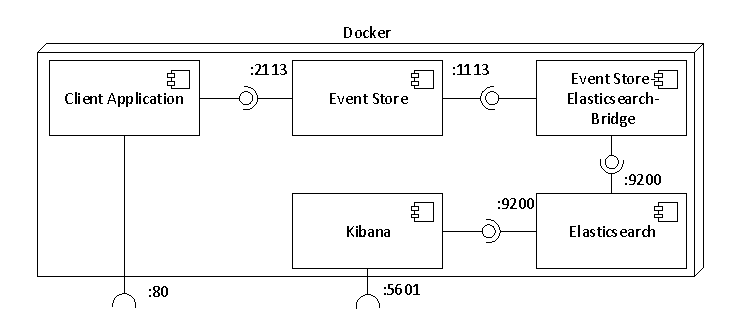
\includegraphics[width=1.2\textwidth]{gfx/docker-architecture.pdf}
}
        \caption[]Component diagram of the final architecture of \ac{IFAS}.{
        Component diagram of the final architecture of \ac{IFAS}.
        Provided interfaces of a service have the number of the connected port attached.
        If a provided interface projects out of the Docker node, the port is exposed outside of the Docker application for other applications to connect with, such as a web browser connecting to Kibana on port 5601.}
        \label{figure:design:architecture}
\end{figure}

\section{Service Orchestration}
\label{sec:implementation:orchestration}

All services run in their own Docker containers in order to facilitate distribution of the system.
Orchestration of the containers is done via \emph{Docker Compose} (short \emph{Compose}), which offers a straightforward way of describing the services of an application and how they interact with each other in one single file (cf. \cref{appendix:code:docker:docker-compose} for the source code of the \texttt{docker-compose.yml} file).
A second Compose file defines the services of the Mattermost application (cf. \cref{appendix:code:docker:mattermost-compose}).

\subsection{Operating the System}

The final setup of \ac{IFAS} enables the following Compose commands, which can either be issued with a specific service name, or without this parameter which causes the command to be executed for all applicable services:

\begin{itemize}
\item Create and start containers for the services defined in the Compose file, via \texttt{docker-compose up [service]}; the additional \texttt{-d} parameter runs the containers in detached mode, i.e. in the background
\item Start the containers that are already created, via \texttt{docker-compose start [service]}
\item Stop and remove containers defined in the Compose file, as well as their volumes and networks, via \texttt{docker-compose down}
\item Stop containers defined in the Compose file, via \texttt{docker-compose stop}
\item Show logging information for a container, via \texttt{docker-compose logs [service]}; the additional \texttt{-f} parameter follows the logs as new ones appear, instead of just printing them once to the  console
\end{itemize}

A user of \ac{IFAS} would usually create and start the containers via \texttt{docker-compose up -d} and then optionally attach to the logs via \texttt{docker-compose logs -f}.
If the system or specific services would have to be taken offline, this could be done via \texttt{docker-compose down}.
For example, the Elasticsearch container would be stopped via \texttt{docker-compose stop elasticsearch}.
Subsequently, the Elasticsearch container would be started again via the \texttt{start} command if no changes to the container are made, e.g. via its service definition, or via the \texttt{up} command if the container has to be recreated.
The \texttt{down} command should only be used if a backup of the relevant Docker volumes was made -- otherwise, all data would be lost.

\subsection{Networking}

Docker allows to assign each container a custom network which allows for virtualization of distinct and separated networks even though the containers all run in the same Docker host.
%This is done via the \texttt{networks} setting for all container definitions, in this case setting the network to \texttt{IFAS-net}.
Two networks were defined for the implemented system: \texttt{IFAS-net} and \texttt{mattermost-net}.

The two networks exist in order to separate \ac{IFAS} functionality more cleanly from the client application -- the only point at which the two interact with each other is when the Mattermost web application sends user feedback events to \ac{IFAS}' Event Store (cf. \cref{figure:implementation:orchestration:network}).
Both networks are default bridge networks, which means that they use a software bridge running in the Docker host to communicate with containers connected to the same bridge.
Communication may occur via another container's IP address or name; for example, the bridge can query data for indexing in Elasticsearch via the base URL \texttt{http://elasticsearch:9200}, where the 9200 denotes the port at which the Elasticsearch container exposes its \ac{HTTP} interface.

This configuration enables Event Store, Elasticsearch, Kibana and the bridge application to freely communicate with each other using the respective service's name.
Hence, neither are the \ac{IFAS} services able to establish communications with a service from the \texttt{mattermost-net} network, nor the other way around.
The exception to this rule is when the Mattermost web application communicates with the Event Store service in the \texttt{IFAS-net} network, but this is only possible as the Event Store service definition explicitly defines that port 2113 shall be exposed publicly.
\ac{IFAS} also exposes the Kibana web application on port 5601 and the Mattermost network serves the chat application on port 80.

\begin{figure}[ht]
\caption[Network diagram of the final architecture of \ac{IFAS}.]{
	Network diagram of the final architecture of \ac{IFAS}.
        Hexagons represent Docker services, the switch icons represent a Docker bridge network.
        Services connected to a bridge network via solid lines can communicate with each other freely within the network.
        Dashed lines represent (possible) connections from the outside of the network, with the opened port being written at the receiving end of the connection.}
        \makebox[\textwidth][c]{
        \includegraphics[width=1.2\textwidth]{gfx/orchestration-network}
}
        \label{figure:implementation:orchestration:network}
\end{figure}

\subsection{Clustering}

Both Event Store and Elasticsearch offer clustering support, but these were deliberately \emph{not} used for this version of \ac{IFAS}.
The reason for this decision is that the performance boost and especially the failover safety introduced by setting up a cluster of Event Store or Elasticsearch nodes is not necessary for \ac{IFAS} at this stage of development, but would introduce additional complexity during implementation and evaluation.
However, this will very likely become relevant when setting the system up for production usage.
For this reason, the following section contains a short description as to how to make use of clustering in \ac{IFAS}.

\paragraph{Clustering in Event Store}
In order to improve availability and read performance, a cluster of multiple Event Store nodes can be set up.
Event Store offers two different types of nodes in clusters: Database nodes and management nodes.
The latter is part of the commercial features of Event Store and thus not further discussed here.
\Cref{appendix:code:implementation:docker:clustering:eventstore} in the appendix shows the source code of a Compose file setting up an Event Store cluster consisting of three database nodes.
This is very similar to the single-node version used in \ac{IFAS}, except for two environment variables which pass the cluster size and its DNS address to every node, so the nodes are able to find each other and vote for a master node.
The documentation\footnote{\url{appendix:code:implementation:docker:clustering:eventstore}} recommends that an odd number of nodes is used, as Event Store uses a quorum based voting protocol (there cannot be a tie if an odd number of nodes is expected to take part in the voting procedure).
When the cluster gets its data via the \ac{HTTP} interface, the documentation further recommends that a load balancer be put in before the cluster in order to distribute the burden equally over all nodes.

\paragraph{Clustering in Elasticsearch}
As described in Elasticsearch's documentation\footnote{\url{https://www.elastic.co/guide/en/elasticsearch/guide/master/distributed-cluster.html}}, an integral concept concerning an Elasticsearch cluster are \emph{shards}.
Shards are worker units that store (parts of) an index.
They are automatically created, enlarged, and shrinked by Elasticsearch as documents are added or removed from the respective index.
Elasticsearch differentiates between \emph{primary} shards and \emph{replica} shards: Each document of an index belongs to exactly one primary shard, replica shards are copies of primary shards.
When a cluster is run in single-node mode, all primary shards are stored on this one node and no replica shards exist.
As soon as a second node is added to the cluster, replica shards are automatically added in order to improve failover safety.
If a third node is added, primary shards are re-allocated from the first node onto the other nodes, thus improving horizontal scalability.
All this happens automatically, as long as all nodes are given the same \texttt{cluster\_name}.
Thus, the Compose configuration is similar to the one for the Event Store cluster.

The Event Store-Elasticsearch bridge is designed to profit from this as well.
Additional instances of the bridge can be created to listen to the same persistent subscription without interfering with each other because Event Store's persistent subscriptions support the competing consumers messaging pattern.
Running multiple bridge instances improves failover safety because the other instances can stand in for the failing one.
Horizontal scalability is also provided on this end, as the bridge instances work independent of each other.
A possible bottleneck exists on the Event Store side, as the persistent subscription's state is managed on the server side.

In conclusion, when running \ac{IFAS} in a production environment, at least two additional Event Store and Elasticsearch nodes should be added by including the respective service definitions to the Compose file.
The service definitions then also have to provide the cluster names and -- for the Event Store cluster -- the cluster's DNS address via environment variables.
In the case of Event Store, a load balancer should also be implemented.
This would form three-node clusters, which immensely improves both failover safety and horizontal scalability.
Additional instances of the Event Store-Elasticsearch bridge can be created as well, if necessary.
